\section{Analyse}
\subsection{Hvordan måler vi hældning?}
Før vi kunne begynde på at lave en hældningssensor blev vi nødt til at finde ud af hvilke muligheder der var hældningsumåling. En af mulighederne var at anvende et pendul eller en libelle. Vi har startede med at udvikle på en prototype af en libellesensor vist på \textit{Figur~\ref{fig:libelle}}.
\begin{figure}[hbpt]
\centering
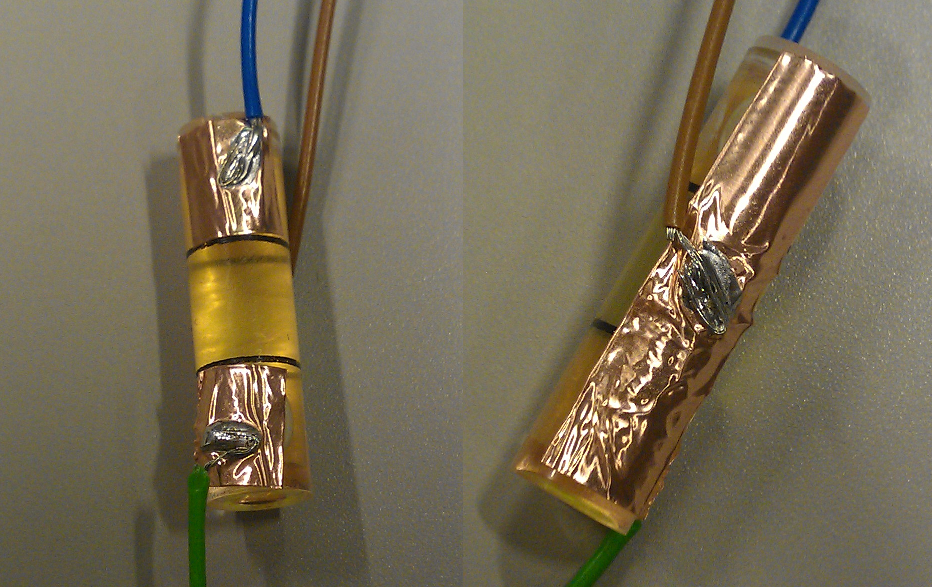
\includegraphics[width=0.4\textwidth]{billeder/libellesensor1}
\caption{Hældningssensor baseret på libelle}
\label{fig:libelle}
\end{figure}
Hældningssensorprototype 1 indeholder 2 højpas filtrer samt en frekvensgenerator og en differensforstærker. Vi kom frem til at libellesensoren har en capacitet på omkring $1*10^{-15}[F]$. Det gør det praktisk umuligt at anvende da vores komponenter i det filter der skulle designes til den færdige sensor, da cutoff frekvens kommer til at være $>3.0[MHz]$. Den høje frekvens giver en stor selvinduktion i vores ledning. Et lavt signal fra hældningssensoren kombineret med stor selvinduktion, gjorde at vi måtte finde en anden løsning.\\
Næste prototype bestod af et potmeter og et pendul. Dog havde potmeteret en for stor friktionsmodstand, der gjorde det upræcist i forhold til vores krav.\\
Vi har gennem et tredje semestersfag fundet ud af at PSoC'en indeholder et accelerometer\footnote{KXSC7-2050 se bilag}. Efter en prototypeopbygning fandt vi ud af at det komponentet opfyldte de krav stille i kravspecifikation. Dog er prototypen implementeret med en '\#define' da databladet er vagt og output varierer mellem PSoCs.
%%%%%%%%%%%%%%%%%%%%
%%% VBTE tis %%%%%%%
%%%%%%%%%%%%%%%%%%%%
\subsubsection{Hvordan måler vi niveauet i vandballasttankene?}
Ultralydsafstandsmålingen blev valgt for at prøve noget ingen havde kendskab til i projektet. Man kunne have valgt at købe en færdiglavet enhed men det blev vurderet at dette ikke gav ret meget faglig erfaring. I e-lab havde de nogle rå tranducere og receivere liggende og der blev derfor valgt at forsøge med at udvikle en ultralydsafstandsmåler. Der blev i starten lavet en del teknologiundersøgelse inden for ultralyden og vi testede tranducere og receivere for at se hvordan de aggerede. Vi fandt at der var en del destruktive reflektioner og vi overvejede at fylde akustisk skum i toppen af tankene, men da det skum vi kunne finde var elektrisk ledende kunne vi ikke anvende det. Jeg kom frem til at et burst skulle sendes for at måle afstanden og en puls på 250$\mu$s blev valgt, hvilket svarer til 10 perioder. Receiverkredsen blev udviklet med viden fra MSE kurset fra sidste semester omkring mixere og operationsforstærkere. Den største erfaring opnået gennem dette forløb må være at man bare, som hovedregel, bare selv skal købe noget der passer til formålet og implementere dette i projektet. Dette giver mere plads til at lave et større system, simplere. Derudover gav det god erfaring i mixerelektronik og ultralydsteknologi, som er meget besværligt at arbejde med.
\fxnote{Johnny Christensen skriver: Epostlen har spist en bussemand}

%%%%%%%%%%%%%%%%%%%%
%%% forsyning %%%%%%
%%%%%%%%%%%%%%%%%%%%
\subsection{Hvordan skal de forskellige modulerne forsynes?}
Da modulerne sidder rundt om i skibbet, skal der overvejes hvordan de kan forsynes. Dette kan ske på flere forskellige måder:
\begin{itemize}
\item Batteri
	\begin{itemize}
	\item Smart da man ungår at trække en ledning med forsyning.
	\item Dette kan være meget problematisk med et batteri, da der ikke vides hvor meget strøm der skal trækkes dvs. stort det skal være. 
	\item Da der i forvejen er en kablet kommunikation, skal der alligevel kabel ud til modulet, derfor kan lige så smart at have en kabelet forsyning.
	\end{itemize}
\item Kablet forsyning \\
Ved at vælge at bruge en kablet forsyning dukker der andre spørgsmål op.
\begin{itemize}
\item F.eks. hvilken forsyningsspænding skal der være.?\\
24V, 230V, 12V, 5V eller noget helt andet..
\end{itemize}
Da der ikke er 100\% kendskab til hvilke forsyning spænding der er på et skib, men nok er 230V AC skal der med stor bruges en strømforsyning til modulerne, da de bruger en lavere spænding. \\
Ved at have en transformator kan spænding evt. komme ned på 24V AC. De 24V AC kan føres ud til modulerne samme med kommunikationen. \\
Ved modulerne kan der bygges en strømforsyning der regulere de 24V AC om til DC. \\
Her kommer der to muliglige strømforsyninger op:
\begin{itemize}
\item En SMPS: \textit{Effektiv, høj virkningsgrad.}
\item En lineær strømforsyning: \textit{Stabil, mellem virkningsgrad}
\end{itemize}
Da virkningsgraden ikke har stor bestydning for produktet, samt erfaringen med SMPS ikke er stor, vil der tages udgangspunkt i en lineær størmforysning.
\end{itemize}
Ved udviklingen af prototypen, kan der overvejes om der skal designes en eller flere strømforsyninger.

\subsection{På hvilken enhed ønsker vi at afvikle programmet KI}
RPi eller ej? Qt4 vs Qt5.\fxnote{Skriv afsnit om RPi og Qt}
\subsection{Hvordan anvendes UART og TCP i Qt-frameworket}
Qt-specifik eller C++? Boost? \fxnote{Skriv afsnit om Qt-frameworket}

\subsection{Jura}
Hvilke lovgivninger findes der på området? Er der et behov for dette? Hvad er de rigtige termer? \fxnote{skriv afsnit om jura}

\subsection{Valg af database}
For at vælge database til systemet blev der kigge på MySQL, Microsoft Acces og en lagring til en tekstfil.\\
Microsoft Acces er et database system der der medfølgende i Microsoft Office pakken. Microsoft Access benytter sit eget format baseret på Access Jet Database Engine. En ulempe ved Microsoft Acces er at den kun fungere under Windows og da systemet skulle alsidigt var dette ikke den bedste løsning. At lagre direkte i en tekst fil blev overvejet da det er meget simpelt at lagre til tekstfiler fra c++ og php kan håndtere at hente fra den. Det kan gå galt ved loading og lagring til filen samtidig med at formater kan blive et problem. \\
Der var i forvejen kendskab til MySQL og dette er et færdig udviklet system til at fungere med webinterfaces og for programmerings sprog som C++ er der udviklet header. Systemet er et system der fungere på mange platforme og løbende bliver udviklet på. På baggrund af dette blev dette system valgt.

